\documentclass{tubaf-article}
\usepackage{graphicx}
\usepackage{subcaption}

\begin{document}
	\title{Scientific Computing Project}
	\subtitle{Winter Semester 2024/2025}
	\author{Lars Wunderlich \and Parsa Besharat \and Toni Sand}
	\date{April 6, 2025}
	\subject{Documentation}
	\publishers{TU Bergakademie Freiberg}
	
	\maketitle
	
	\tableofcontents
	
	\newpage
	
	\section{Task}
	
	The goal of this project was to code the model of a convolutional neural network and train it for the task of classifying images which consists of assigning them to one of 10 possible classes. The used training images are self-generated by the students of this course and collected into a database. A detailed description of the used training data can be found in chapter \ref{dataset}, whereas the architecture of the network is explained in chapter \ref{architecture}. Especially, the network should also be able to classify new images correctly. In chapter \ref{training} we talk about the training process and the tuning of hyperparameters like learning rate, batch size or optimizer by using k-fold cross-validation. At the end in chapter \ref{results}, we evaluate the result of our work by looking at several performance measurements like the confusion matrix and the loss and accuracy curves. Finally, we discuss approaches for improvement.
	
	\section{Description of the Data Set}
	\label{dataset}
	The data set that is used for training the network consists of 10 classes of images. These are
	\begin{center}
		\begin{tabular}{ c c c c c }
			1. bottles & 2. mugs/cups & 3. spoons & 4. knifes & 5. forks \\ 
			6. shoes & 7. t-shirts & 8. plants & 9. chairs & 10. bikes    
		\end{tabular}
	\end{center}
	Every student had to contribute to this database by generating 15-20 pictures of pairwise disjoint objects for each class. In total there are approximately 400 images per class which yield a database of almost 4000 images. 
	\begin{figure}[h!]
		\centering
		% Erstes Bild
		\begin{subfigure}[b]{0.3\textwidth}
			\centering
			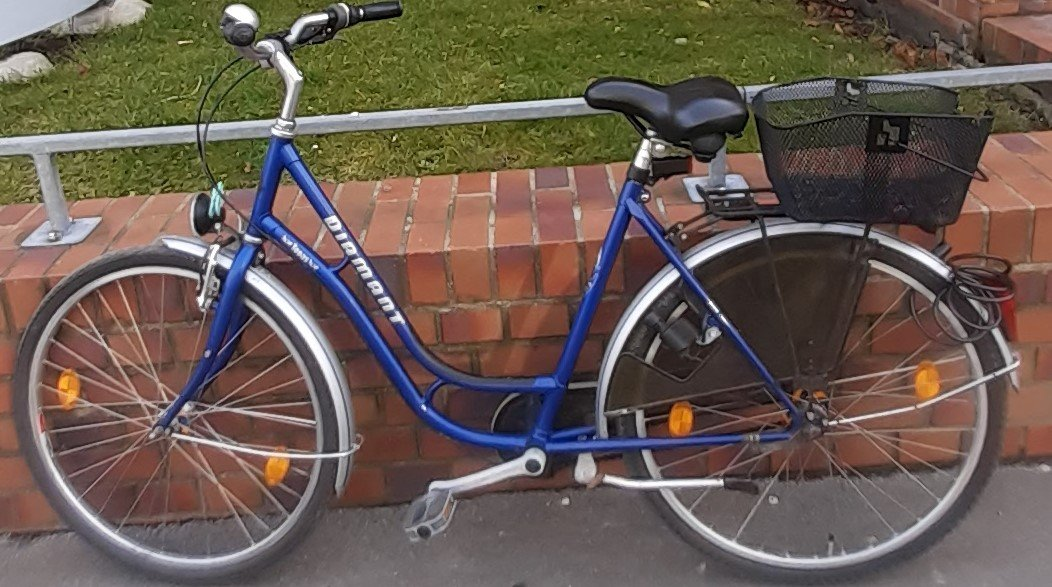
\includegraphics[width=\textwidth]{ex1.jpeg}
			\caption{10. bikes}
			\label{fig:bild1}
		\end{subfigure}
		\hfill
		% Zweites Bild
		\begin{subfigure}[b]{0.3\textwidth}
			\centering
			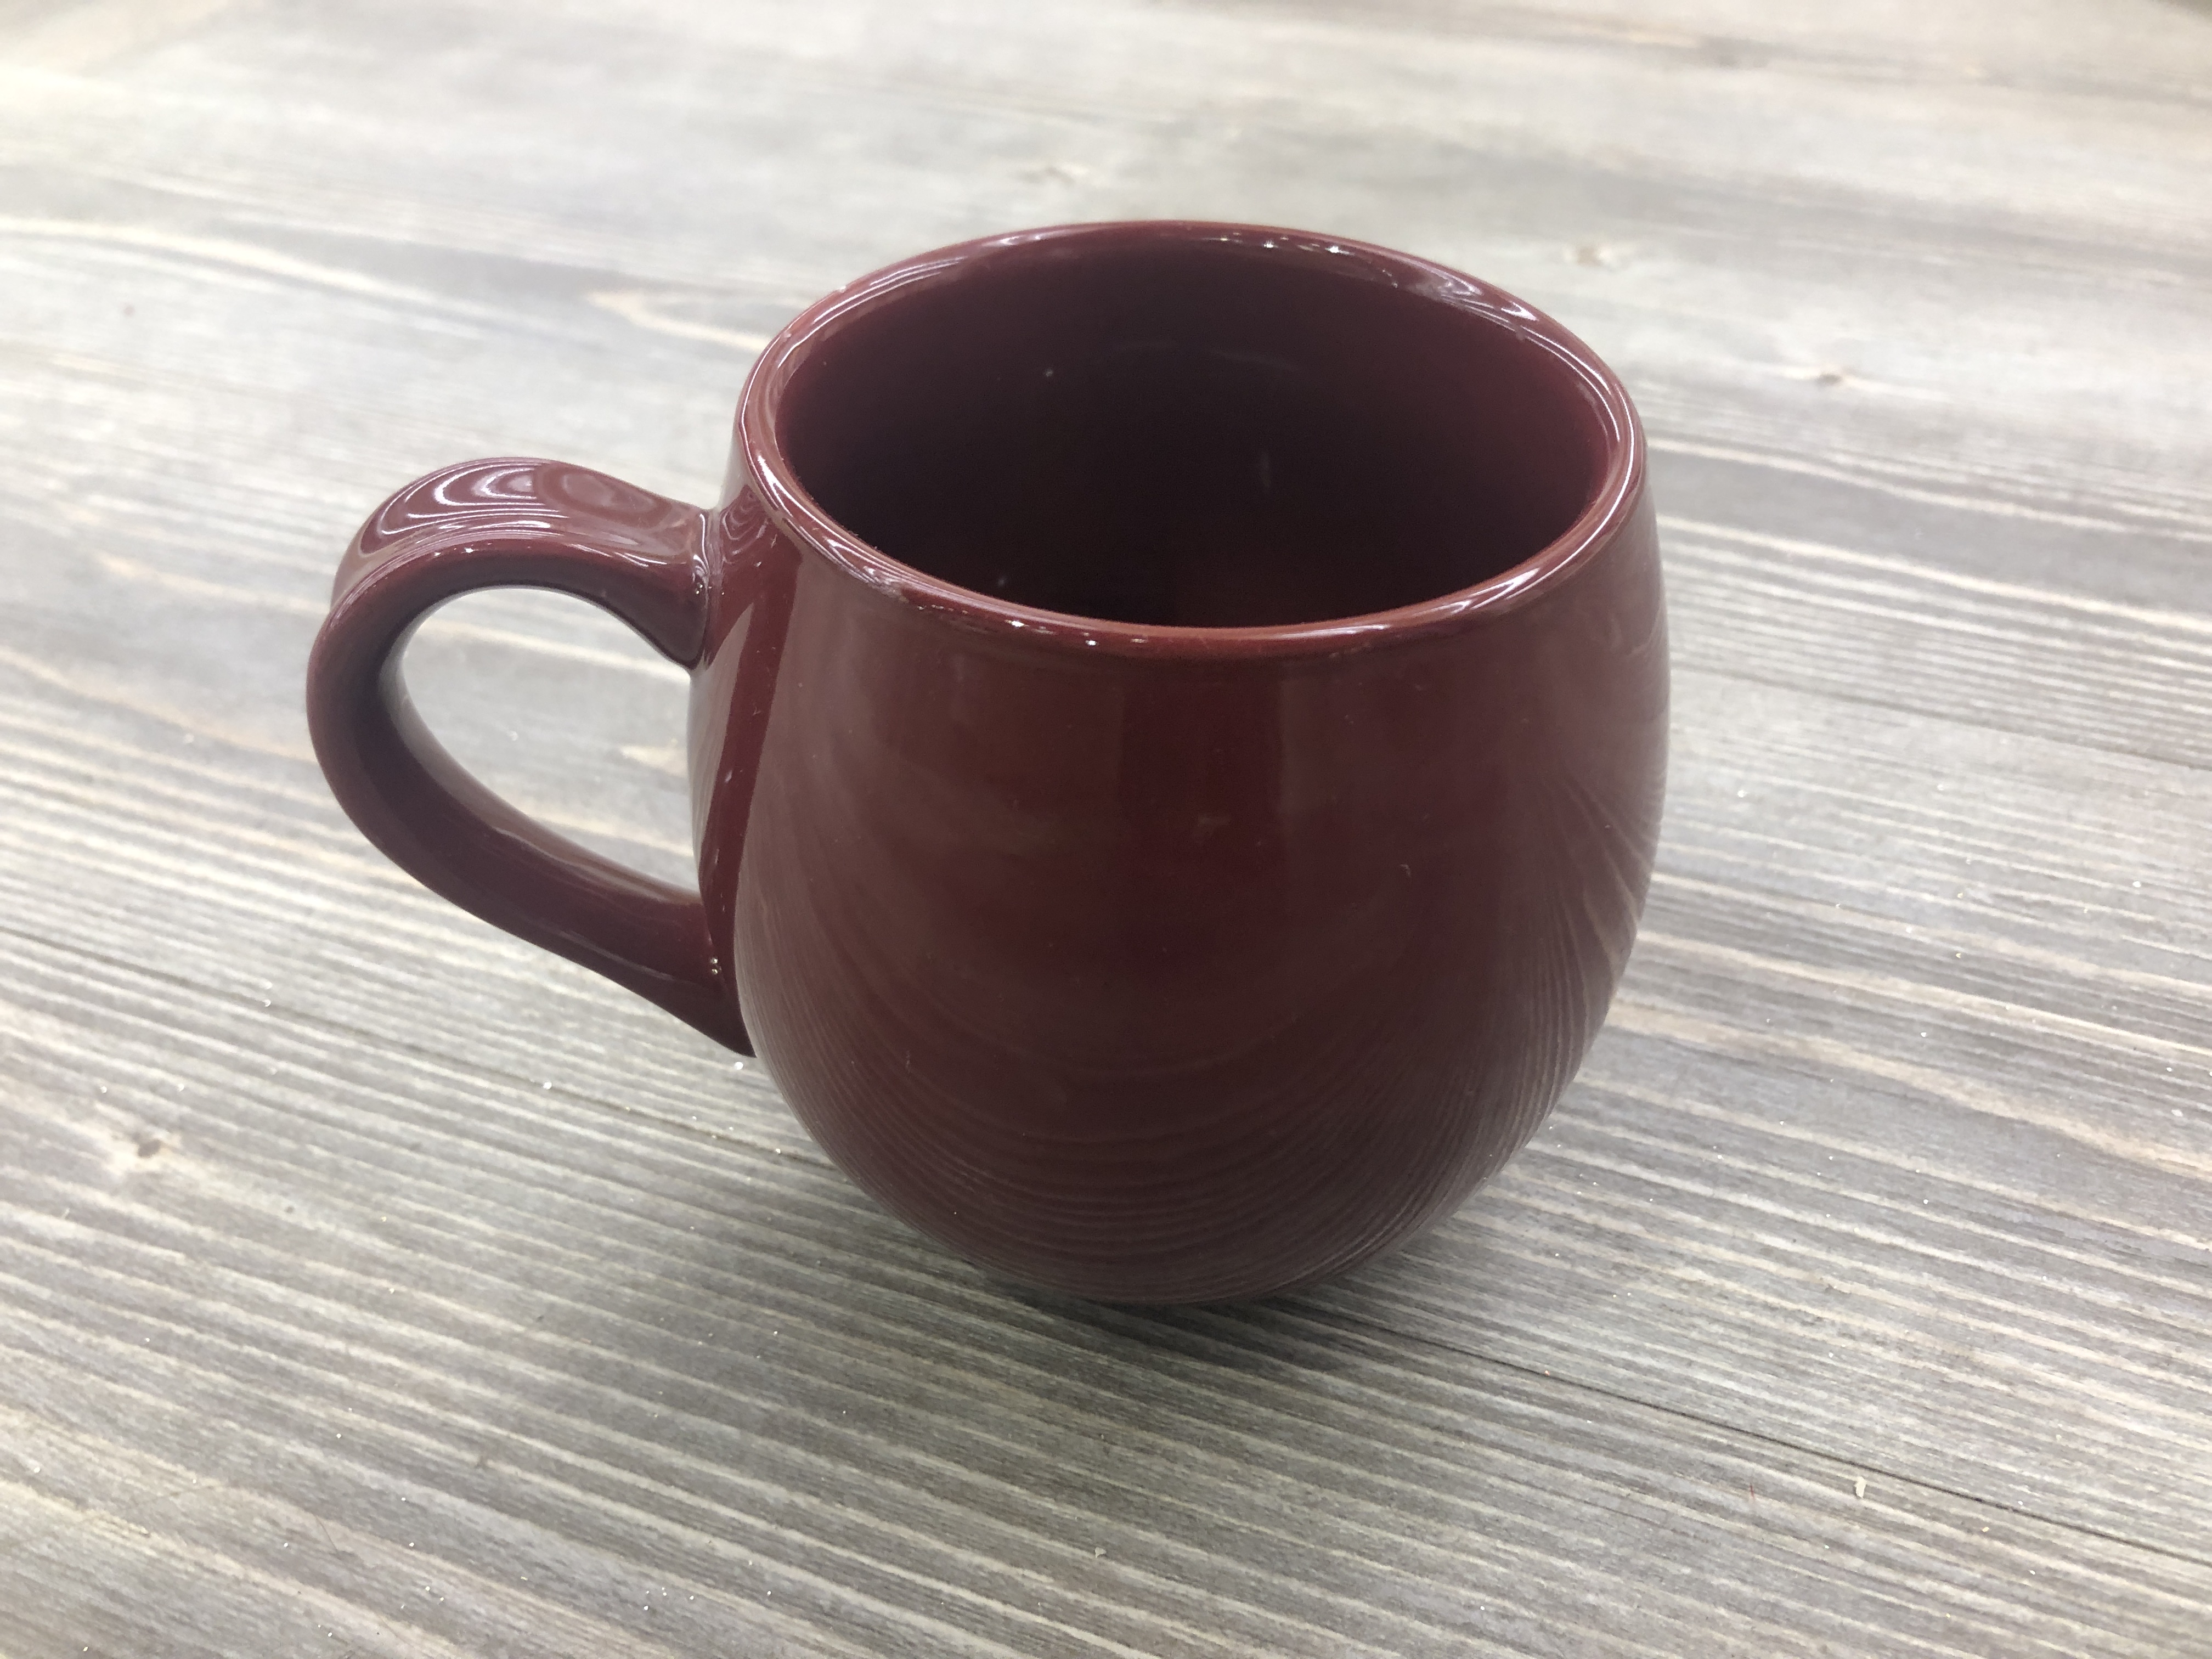
\includegraphics[width=\textwidth]{ex3.jpeg}
			\caption{2. mugs/cups}
			\label{fig:bild2}
		\end{subfigure}
		\hfill
		% Drittes Bild
		\begin{subfigure}[b]{0.3\textwidth}
			\centering
			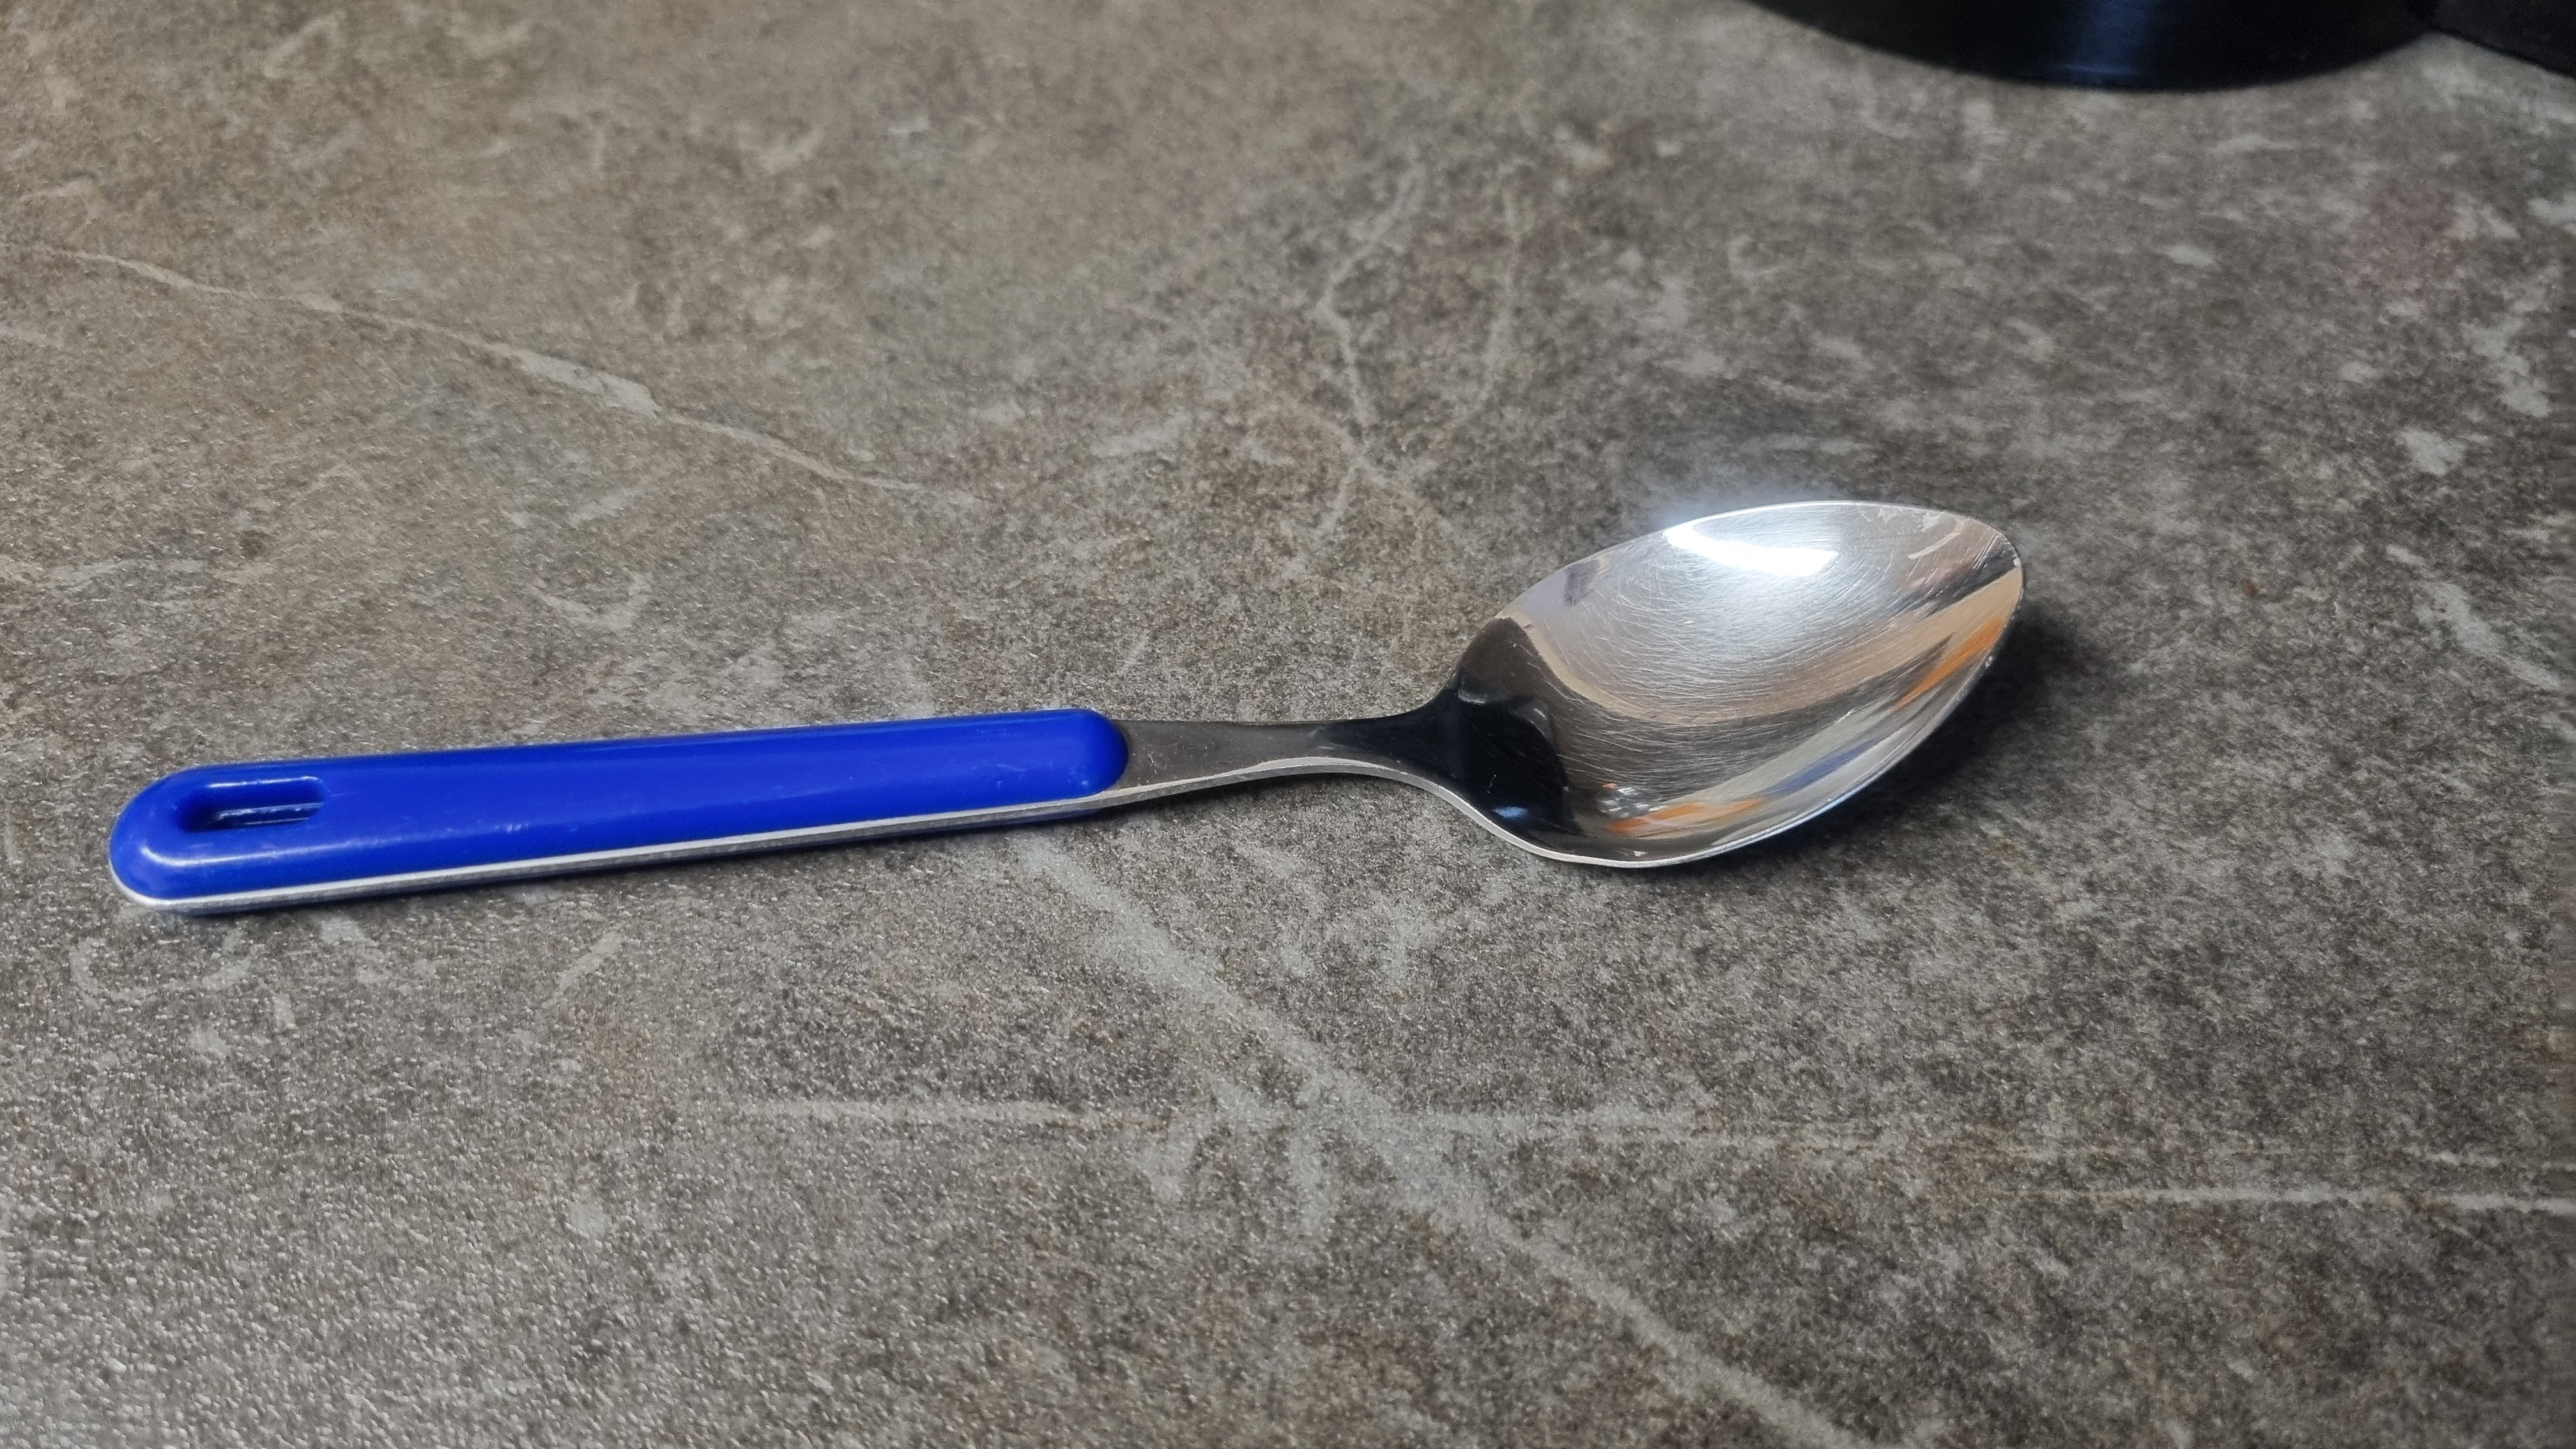
\includegraphics[width=\textwidth]{ex2.jpeg}
			\caption{3. spoons}
			\label{fig:bild2}
		\end{subfigure}
		\hfill
		\caption{Example images of some classes}
		\label{fig:nebeneinander}
	\end{figure}
	In the next step the image database was normalized \emph{(by doing...)} to make the training possible. To enlarge the database and improve the training process, we used data augmentation techniques in the following manner \emph{(insert detailed description...)}. \\
	TODO: insert example augmented images \\
	As a result of this preprocessing procedure, we got a database of ... images for the training and testing of our neural network.
	
	
	\section{Architecture of the Network}
	\label{architecture}
	
	\section{Training}
	\label{training}
	
	\section{Results}
	\label{results}
	
\end{document}
